\documentclass{book}
\usepackage[utf8]{inputenc}
\usepackage{amsmath}
\usepackage{amssymb}
\usepackage{enumitem}
\usepackage{geometry}
\usepackage{booktabs}    % \toprule, \midrule, \bottomrule
\usepackage{tabularx}    % colonne X che si adattano alla linewidth
\usepackage{ragged2e}    % \RaggedRight per testi giustificati in X
\usepackage{caption}
\geometry{a4paper, margin=1in}
\usepackage{graphicx}
\usepackage{xcolor}
% Redefine the caption format to remove "Figure" and the number
\captionsetup[figure]{labelformat=empty}
\title{%
	Reti di calcolatori e internet\\
	\small Appunti}
\author{Alessandro Ferro}
\renewcommand{\chaptername}{Capitolo}
\date{}

\begin{document}

\maketitle
	
\chapter*{Introduzione}
Questi appunti, presi dal libro "Reti di Calcolatori e Internet - un approccio Top Down" (Kurose, Ross, 7th edition) sono parziali in quanto una parte sono presi a penna. La numerazione dei capitoli, sezioni e paragrafi segue quella del libro.
		
\chapter{Reti di calcolatori e Internet}
	
[Le sezioni 1.1 e 1.2 sono scritte a penna sul quaderno]
	
\section*{1.3 Il nucleo della rete}
	
\subsection*{1.3.2 Commutazione di circuito}
Per spostare i dati in una rete esistono due approcci: commutazione di pacchetto e commutazione di circuito. 
	
Nelle reti a commutazione di circuito, le risorse necessarie sono allocate per l'intera durata della comunicazione tra i sistemi periferici. Nelle reti a commutazione di pacchetto, invece, tali risorse non sono riservate e sono allocate in funzione della necessità della rete.
	
Le reti telefoniche sono esempi di rete a commutazione di circuito in quanto il canale resta aperto anche in assenza di comunicazione.
	
Quando la rete stabilisce un circuito, viene riservata anche una certa larghezza di banda, pertanto, il mittente può trasferire i dai a una velocità costante garantita.
	
D'inverso, quando un host invia un pacchetto a un altro host su una rete a commutazione di pacchetto, esso viene immesso nella rete senza che vengano ad esso riservate risorse.
	
\subsubsection{Multiplexing nelle reti a commutazione di circuito}
In una rete a commutazione di circuito può essere implementato il multiplexing, ovvero l'utilizzo dello stesso mezzo trasmissivo da più utenti.
	
Il multiplexing viene implementato tramite:
	
\begin{itemize}
	\item Suddivisione di frequenza: lo spettro di frequenza di un collegamento viene suddiviso tra le connessioni stabilite. Ciò, ad esempio, è il caso di walkie-talkie che comunicano su un circuito a una frequenza diversa da altri walkie-talkie che comunicano sullo stesso circuito.
	\item Suddivisione di tempo: quando la rete stabilisce una connessione a commutazione di circuito, assegna degli slot temporali per ogni sessione.
\end{itemize}

\subsubsection{Confronto tra commutazione di pacchetto e commutazione di circuito}
I denigratori della commutazione di pacchetto sostengono che quest'ultimo mal si adatti alle applicazioni in tempo reale a causa dei suoi ritardi variabili e non deterministici. I suoi sostenitori, invece, affermano che la commutazione di pacchetto non soltanto offra una migliore condivisione della larghezza di banda, ma è anche più semplice, efficiente ed economica.
	
La commutazione di pacchetto risulta essere più efficiente perché la commutazione di circuito prealloca l'uso del collegamento trasmissivo indipendentemente dalla richiesta necessaria, con collegamenti garantiti ma potenzialmente non necessari. D'altro canto la commutazione di pacchetto alloca le risorse su richiesta.
	
\subsection*{1.3.3 Una rete di reti}
Gli ISP si distinguono per la copertura geografica: gli ISP di accesso, che forniscono Internet direttamente all'utente finale, sono connessi agli ISP regionali che a loro volta sono connessi agli ISP di primo livello (cosiddetti ISP globali). Tale configurazione permette a tutti i nodi della rete di essere in comunicazione.
	
Per ridurre i costi una coppia di ISP vicini e di pari livello gerarchico può fare uso di peering, cioè connettere direttamente le loro reti in modo tale che il traffico passi direttamente tra di loro anziché passare per un intermediario.
	
\section*{1.4 Ritardi, perdite e throughput nelle reti a commutazione di pacchetto}
Idealmente, vorremmo che i servizi Internet siano in grado di spostare dati tra due sistemi periferici istantaneamente e senza nessuna perdita dati. Ciò, ovviamente, non è fattibile nella realtà: il throughput è necessariamente limitato, ci possono essere ritardi e si potrebbero perdere pacchetti.
	
\subsection*{1.4.1 Panoramica del ritardo nelle reti a commutazione di pacchetto}
Un pacchetto parte da un host, passa una serie di router e conclude il viaggio in un altro host. In ciascun nodo lungo il percorso (inclusi sorgente e destinazione) il pacchetto subisce vari tipi di ritardo. I principali ritardi sono dovuti al ritardo di elaborazione, ritardo di accodamento, ritardo di trasmissione e ritardo di propagazione che complessivamente formano il ritardo totale di nodo. 
	
La figura 1.16 mostra un ottimo schema che riassume i tipi di ritardo.
	
\subsubsection{Ritardo di elaborazione}
Il tempo richiesto per esaminare l'intestazione del pacchetto e per determinare dove dirigerlo, nonché il tempo richiesto per controllare eventuali errori al suo interno fa parte del ritardo di elaborazione.
	
\subsubsection{Ritardo di accodamento}
Una volta in coda, il pacchetto subisce un ritardo di accodamento mentre attende la trasmissione sul collegamento. Ne abbiamo già parlato in 1.3.1 "ritardi di accodamento e perdita di pacchetti"
	
\subsubsection{Ritardo di trasmissione}
Sia $L$ la lunghezza del pacchetto in bit e $R$ la velocità di trasmissione in bps dal router A al router B, il ritardo di trasmissione è $\frac{L}{R}$ secondi e risulta essere il tempo richiesto per trasmettere tutti i bit del pacchetto sul collegamento.

\subsubsection{Ritardo di propagazione}
Una volta immesso sul collegamento, il pacchetto deve propagarsi fino al successivo nodo della rete. Questo tempo si chiama ritardo di propagazione.
Il ritardo di propagazione è dato da $d/v$ dove $d$ è la distanza tra i due router e $v$ è la velocità di propagazione nel collegamento (in $m/s$). Questo ritardo è puramente fisico: indica quanto tempo impiega un singolo bit a “viaggiare” dal mittente al destinatario una volta che è stato trasmesso. Questo ritardo solitamente è trascurabile. 
	
\subsubsection{Confronto tra ritardi di trasmissione e di propagazione}
Il ritardo di trasmissione è la quantità di tempo impiegata dal router per trasmettere in uscita il pacchetto ed è funzione della lunghezza del pacchetto e della velocità di trasmissione sul collegamento, ma non ha niente a che fare con la distanza tra i due router. Come detto poc'anzi, è il tempo richiesto per trasmettere tutti i bit del pacchetto sul collegamento.
	
Il ritardo di propagazione, invece, è il tempo richiesto per la propagazione di un solo bit da un router a quello successivo ed è funzione della distanza tra i due router e della velocità di propagazione nel mezzo trasmissivo ma non ha niente a che fare con la dimensione del pacchetto o la velocità di trasmissione.
	
Nota come velocità di trasmissione $\neq$ velocità di propagazione.

\begin{table}[ht]
	\centering
	\resizebox{\textwidth}{!}{%
		\begin{tabular}{r l p{0.6\textwidth} c}
			\hline
			& \textbf{Nome (simbolo)} & \textbf{Significato} & \textbf{Unità tipica} \\ 
			\hline
			1 & \textbf{Velocità di propagazione} ($v$) &
			Velocità con cui \textbf{un segnale elettrico/ottico} si propaga fisicamente lungo il mezzo (rame, fibra, aria, ecc.).&
			metri/secondo (m/s) \\[6pt]
			2 & \textbf{Velocità di trasmissione} (o \textit{data rate}) ($R$) &
			Velocità con cui \textbf{i bit vengono trasmessi} sul collegamento, cioè quanti bit al secondo vengono ``iniettati'' nel canale. &
			bit/secondo (bps) \\
			\hline
		\end{tabular}%
	}
	\caption{Confronto tra velocità di propagazione e velocità di trasmissione.}
\end{table}

\subsubsection{Formula}
Siano $d_{elab}$, $d_{acc}$, $d_{tra}$, $d_{prop}$, i ritardi, rispettivamente di elaborazione, accodamento, trasmissione e propagazione. Allora, il ritardo totale di un nodo è dato da:
$$ d_{elab} + d_{acc} + d_{tra} + d_{prop} $$ 

\subsection*{1.4.2 Ritardo di accodamento e perdita di pacchetti}
A differenza degli altri tre ritardi, quello di accodamento può variare da pacchetto a pacchetto. Ciò vuol dire che mentre elaborazione, trasmissione e propagazione sono costanti per ogni pacchetto che viaggia su quella specifica tratta, il ritardo di accodamento è variabile. Per tale motivo, nel caratterizzare il ritardo di accodamento si fa uso di misure statistiche quali il ritardo di accodamento medio e la sua varianza.

Denotiamo con $a$ la velocità di arrivo di pacchetti nella coda espressa in pacchetti al secondo, $R$ la velocità di trasmissione alla quale i bit vengono trasmessi in uscita alla coda espressa in bit al secondo e supponiamo che tutti i pacchetti abbiano dimensione $L$ bit. Pertanto arrivano al nodo $La$ bit/s.

Con $La/R$ si denota l'intensità di traffico e il risultato è un numero adimensionale (es. $\frac{500bps}{250bps} = 2$)
	
\begin{itemize}
	\item \textbf{(1)} Se $La/R > 1$ vuol dire che stanno entrando più pacchetti di quanti il nodo può trasferirne in uscita e la coda cresce verso $\infty$ bit. 
	
	Questo perché $\frac{La}{R} > 1$ implica che $La > R$

	\item \textbf{(2)} Se $La/R \leq 1$ succede quanto segue: Innanzitutto nota che se ogni pacchetto ha dimensione $L$ vuol dire che il nodo impiega $\frac{L}{R}$ secondi per smaltirlo. Ora ipotizziamo che $N$ pacchetti giungano simultaneamente ogni $N(\frac{L}{R})$ secondi. Se ogni pacchetto viene smaltito ogni $\frac{L}{R}$ secondi, in $N(\frac{L}{R})$ secondi ne vengono smaltiti esattamente $N$. 
	
	In questo caso il primo pacchetto inizia a uscire dalla coda immediatamente, il secondo pacchetto deve aspettare $L/R$ secondi prima che il suo primo bit esca dalla coda, il terzo deve aspettare $2 * \frac{L}{R}$, il quarto deve aspettare $3 * \frac{L}{R}$ secondi e così via. Più in generale, il pacchetto N° deve aspettare $(N-1) * \frac{L}{R}$.
	
	Per rendere più chiaro il concetto facciamo un esempio. Si supponga che arrivino 10 pacchetti all'istante 0 ognuno grande 50bit con una velocità di trasmissione $R$ pari a  1000bit/s. Il primo pacchetto inizia a uscire dalla coda subito, ma il primo bit del secondo pacchetto deve aspettare $\frac{L}{R} = \frac{50}{1000} = 0.05s$ prima che l'intero pacchetto precedente sia completamente uscito. Il decimo pacchetto deve aspettare $(9) * 0.05 = 0.45s$ e, nel momento in cui il suo trasferimento sul collegamento sarà terminato, a tempo $0.5$, ne subentrano altri 10, di cui il primo non deve aspettare nulla prima che inizia a essere trasferito.

	Ciò dimostra che la condizione $La/R \leq 1$, non garantisce assenza di attese.

\end{itemize}
	
\subsubsection{Perdita di pacchetti}
La quantità di pacchetti perduti aumenta in proporzione all'intensità di traffico in quanto la coda potrebbe non essere abbastanza capiente per soddisfare la richiesta. Pertanto, le prestazioni di un nodo sono misurate non solo in termini di ritardo ma anche dalla probabilità di perdita di pacchetti.

\subsubsection{1.4.3 Ritardo end to end}
Nella sottosezione 1.3.1 (paragrafo "trasmissione store e forward") abbiamo detto che, supponendo di avere N-1 nodi tra sorgente e destinazione (e quindi N collegamenti) il ritardo end-to-end è
$$d_{e2e} = N(d_{trasmissione}) = N(\frac{L}{R})$$

ma prendevamo in considerazione solo il ritardo di trasmissione. La formula generale è 
$$d_{e2e} = N(d_{elab} + d_{accodamento} + d_{trasmissione} + d_{prop})$$

\subsubsection{Traceroute}
Traceroute è un programma eseguibile su qualsiasi host di Internet. Quando l'utente specifica il nome di un host di destinazione, il programma invia pacchetti speciali verso di essa, che, durante il loro percorso, passano attraverso una serie di router. Quando uno di questi router riceve questo pacchetto speciale, invia un messaggio che torna alla destinazione che contiene il nome e l'indirizzo del router.

Il funzionamento è il seguente: Supponiamo di avere N-1 router dalla sorgente alla destinazione. La sorgente invia N pacchetti ognuno dei quali contiene l'indirizzo della destinazione. Quando l' n-esimo router riceve il pacchetto marcato come n, anziché indirizzarlo verso la destinazione risponde al mittente come poc'anzi descritto. L'N-esimo pacchetto, che raggiunge la destinazione, invita anche quest'ultima a rispondere.

In questo modo l'origine può ricostruire il percorso intrapreso dai pacchetti ed è inoltre in grado di determinare i ritardi per ogni nodo.

\subsubsection{Sistemi periferici, applicazioni e altri ritardi}
Oltre ai ritardi descritti nelle sezioni precedenti, si potrebbero manifestare ulteriori ritardi nei sistemi periferici. A titolo esemplificativo, un sistema periferico può volontariamente ritardare la sua trasmissione in quanto condivide il mezzo trasmissivo con altri sistemi periferici.

Un altro esempio è nel VoIP: In VoIP il mittente deve prima di tutto riempire il pacchetto con conversazione digitalizzata prima di inviarlo su Internet. Questo tempo per riempire un pacchetto è detto ritardo di pacchettizzazione.

\subsection*{1.4.4 Throughput nelle reti di calcolatori}
Un'altra misura critica delle prestazioni in una rete di calcolatori è il throughput end-to-end.

Consideriamo un trasferimento di file da A a B. Il throughput istantaneo in ogni istante di tempo è la velocità di bit/s alla quale B sta ricevendo il file. È misurato in B e non in A in quanto è l'unico modo per individuare la velocità effettiva di trasferimento dopo tutti i ritardi e colli di bottiglia che intercorrono nel percorso.

Se il file consiste di F bit e il trasferimento richiede T secondi affinché la destinazione riceva tutti i bit, allora il throughput medio è $F/T$ bit/s.

Supponiamo che A e B si stiano trasferendo un file e che tra di loro ci sia un router C. Supponiamo $R_{1}$ essere il throughput da A a C e $R_{2}$ il throughput da C a B. Se $R_{1} \leq R_{2}$ allora la velocità di collegamento da A a B (throughput end to end) è $R_{1}$ ma se $R_{1} > R_{2} $ la velocità di collegamento è $R_{2} $ in quanto il router fa da collo di bottiglia. Quindi il throughput end to end è $MIN(R_{1}, R_{2})$ o più in generale $MIN(R_{1}, ..., R_{n+1})$
se ci sono $n$ router.

\section*{1.5 Livelli dei protocolli e loro modelli di servizio} 
\subsection*{1.5.1 Architettura a livelli}
Un'architettura a livelli consente di discutere e analizzare una parte specifica e ben definita di un sistema complesso. Ciò permette di introdurre un ulteriore vantaggio: la modularità, che rende molto più facile cambiare l'implementazione di un servizio fornito da un determinato livello. Fino a quando il livello fornisce lo stesso servizio allo strato superiore e utilizza gli stessi servizi dello strato inferiore, la parte rimanente del sistema (ovvero gli altri livelli) rimane invariata al variare dell'implementazione del livello.

\subsubsection{Stratificazione dei protocolli}
I protocolli, nonché l'hardware e il software che li implementano, sono organizzati in livelli. Ciascun protocollo appartiene a uno dei livelli. Ogni livello fornisce il suo servizio $(1)$ effettuando determinate azioni all'interno del livello stesso e $(2)$ utilizzando i servizi del livello immediatamente inferiore (se c'è).

Un livello può essere implementato via hardware, software o con una combinazione di essi.

L'insieme dei protocolli di tutti i livelli viene chiamato pila di protocolli. Internet è formato da una pila a 5 livelli. Questi livelli sono: fisico, collegamento, rete, trasporto e applicazione. In ambito accademico si studia anche la pila a 7 livelli denominata ISO/OSI.

Un protocollo, per sua natura, serve per scambiare messaggi. Pertanto, un protocollo "vive" su più sistemi di rete.

Degli svantaggi dell'architettura a strati sono la possibilità che un livello duplichi le funzionalità di un livello inferiore e che un livello possa prelevare informazioni da altri livelli bypassandone i servizi esposti. Ciò viola lo scopo della separazione tra livelli.

\subsubsection{Livello di applicazione}
Il livello di applicazione è la sede dei protocolli usati dalle applicazioni di rete. Alcuni dei protocolli a questo livello sono HTTP, SMTP e FTP. I pacchetti di informazione del livello di rete vengono denominati messaggi.

\subsubsection{Livello di trasporto}
Il livello di trasporto trasferisce i messaggi del livello di applicazione. Vi sono due protocolli di trasporto: TCP e UDP.

\begin{itemize}
	\item TCP: fornisce alle applicazioni un servizio orientato alla connessione (cioè l'utente deve stabilire una connessione, usarla e quindi rilasciarla), garantisce la consegna dei messaggi di applicazione e il loro ordine. Gestisce il controllo di flusso (ovvero la corrispondenza tra le velocità del mittente e destinatario) e ha inoltre un controllo di congestione della rete.
	
	\item UDP: questo protocollo è molto semplice. Non è orientato alla connessione e non garantisce affidabilità, controllo di flusso e controllo della congestione.
\end{itemize}
I pacchetti a livello di trasporto sono denominati segmenti.

\subsubsection{Livello di rete}
Il livello di rete si occupa di trasferire i pacchetti a livello di rete, detti datagrammi, da un host a un altro.

Il livello di trasporto passa al livello di rete il proprio segmento e un indirizzo di destinazione.

Il livello di rete comprende il protocollo IP.


\subsubsection{Livello di collegamento}
Per trasferire un pacchetto da un nodo a quello successivo sul percorso, il livello di rete si affida ai servizi del livello di collegamento. Esempi di protocolli a livello di collegamento includono Ethernet e WiFi.

Un datagramma potrebbe essere gestito da differenti protocolli a livello di collegamento lungo le diverse tratte che costituiscono il suo percorso.

Chiameremo frame i pacchetti a livello di collegamento.

\subsubsection{Livello fisico}
Mentre il compito del livello di collegamento è spostare frame tra nodi adiacenti, il ruolo del livello fisico è spostare i singoli bit. I protocolli di questo livello dipendono dall'effettivo mezzo trasmissivo.

\subsection*{1.5.2 Incapsulamento}
Dalla sorgente, i dati scendono lungo la pila dei protocolli e vi risalgono nella destinazione. Nei commutatori, i dati scendono e salgono fino a un determinato livello: per i commutatori a livello di collegamento fino al livello 2, per i router fino al livello 3. Gli host implementano tutti e cinque i livelli.

In altre parole, presso un host mittente, un messaggio a livello di applicazione viene passato al livello di trasporto. Questo livello prende il messaggio e gli concatena informazioni aggiuntive (le informazioni di intestazioni) che verranno utilizzate dal protocollo di trasporto nell'host ricevente. Messaggio livello applicazione + intestazioni del protocollo di trasporto costituiscono il segmento.

Il protocollo di trasporto passa il segmento al livello di rete, il quale gli concatena le proprie intestazioni, formando il datagramma e così via scendendo nella pila.

Quindi a ciascun livello il pacchetto ha due tipi di campi: quello di intestazione e quello di payload (il carico utile). Il payload è tipicamente un pacchetto proveniente dal livello superiore.

\chapter{Livello di applicazione}
Le applicazioni sono la ragion d'essere delle reti di calcolatori. Senza di esse predisporre una rete sarebbe inutile.

\section*{2.1 Principi delle applicazioni di rete}
I programmi che fanno uso del livello Applicazione sono eseguiti sui sistemi periferici che comunicano tra loro via rete. Esempi di programmi sono i browser e i web server. I programmatori delle applicazioni a livello di rete non hanno bisogno di scrivere software che viene eseguito sui commutatori

\subsection*{2.1.1 Architettura delle applicazioni di rete}
Per lo sviluppatore di applicazioni l'architettura di rete è fissa e fornisce alle applicazioni uno specifico insieme di servizi. Il compito dello sviluppatore è progettare l'applicazione. Egli deve scegliere tra utilizzare l'architettura client-server o P2P (peer-to-peer).

Nell'architettura client-server vi è un host sempre attivo, chiamato server, che risponde alle richieste di servizi da altri host, detti client. I client non si connettono direttamente fra loro.

In un'architettura P2P si sfrutta invece la comunicazione diretta di host, chiamati peer, che a differenza di un server centralizzato possono (e spesso lo sono) collegati in maniera intermittente. I peer non appartengono a un fornitore di servizi ma appartengono agli utenti. Uno dei punti di forza dell'architettura P2P è la sua intrinseca scalabilità e sono anche economicamente convenienti perché non richiedono server prestanti nè una banda elevata.

Alcune applicazioni presentano un'architettura ibrida, combinando sia elementi P2P che client-server.

\subsection*{2.1.2 Processi comunicanti}
I processi su due sistemi terminali comunicano scambiandosi messaggi attraverso la rete. Il processo mittente crea e invia messaggi sulla rete e il processo destinatario li riceve e, quando previsto, invia messaggi di risposta.

\subsubsection*{Processi client e server}
Per ciascuna coppia di processi comunicanti ne etichettiamo uno come client e l'altro come server. In alcune applicazioni un processo può essere sia client che server (come ad esempio in un programma P2P). Nonostante ciò possiamo comunque etichettarli basandoci sul contesto di una specifica sessione.

Un processo che richiede il servizio o le informazioni è indicato come client mentre quello che eroga il servizio o procura le informazioni è detto server.

\subsubsection*{L'interfaccia tra il processo e la rete}
Ogni messaggio inviato da un processo a un altro remoto deve passare attraverso la rete sottostante. Il processo presuppone l'esistenza di un'infrastruttura esterna che trasporterà il messaggio attraverso la rete.

Un processo invia messaggi nella rete e riceve messaggi dalla rete attraverso un'interfaccia software detta socket. Una socket è l'interfaccia tra il livello di applicazione e quello di trasporto all'interno di un host. Viene chiamata anche API tra l'applicazione e la rete.

Il progettista di un'applicazione può (1) scegliere il protocollo di trasporto e (2) talvolta determinare alcuni parametri a livello di trasporto.

\subsubsection*{Indirizzamento}
I processi riceventi devono poter avere un indirizzo per ricevere i messaggi inviati da un processo in esecuzione su un altro host. Per identificare un processo ricevente è necessario specificare due informazioni: (1) l'indirizzo dell'host e (2) un identificatore del processo ricevente sull'host di destinazione. Il punto (2) serve perché su un host potrebbero esserci più processi in esecuzione simultaneamente.

In Internet gli host vengono identificati attraverso un indirizzo IP, composto da 32 bit, che per il momento, possiamo pensare che identificano univocamente un host. Il processo mittente deve anche identificare il processo destinatario, più specificatamente, la socket che deve ricevere il dato. Un numero di porta di destinazione assolve questo compito. Alle applicazioni più note sono stati assegnati numeri di porta specifici.

\subsection*{2.1.3 Servizi di trasporto disponibili per le applicazioni}
Il protocollo a livello di trasporto ha la responsabilità di consegnare i messaggi alla socket del processo ricevente. I protocolli di trasporto lo possiamo classificare in 4 dimensioni: trasferimento dati affidabile, throughput, temporizzazione e sicurezza

\subsubsection*{Trasferimento dati affidabile}
In alcune applicazioni la perdita di informazioni potrebbe causare gravi conseguenze. Dunque, per supportare tali applicazioni occorre garantire che i dati inviati siano consegnati corretti e completi. Se un protocollo fornisce ciò si dice che fornisce un trasferimento dati affidabile.

In questo caso il processo mittente può passare alla socket i messaggi e sapere con assoluta certezza che verranno recapitati al processo ricevente.

Invece, le applicazioni che tollerano le perdite sono le applicazioni audio/video.

\subsubsection*{Throughput}
Un protocollo a livello di trasporto potrebbe fornire un throughput garantito. Con tale servizio l'applicazione potrebbe chiedere che il throughput sia almeno di $r$ bps.

Le applicazioni che hanno requisiti di throughput si dicono applicazioni sensibili alla banda, che si oppongono alle cosiddette applicazioni elastiche che possono funzionare anche senza garanzia di throughput.

\subsubsection*{Temporizzazione}
Un protocollo a livello di trasporto potrebbe anche fornire garanzie di temporizzazione, ovvero garantire che ogni bit che il mittente invia venga consegnato al destinatario in non più di $t$ secondi.

\subsubsection*{Sicurezza}
Un protocollo a livello di trasporto può fornire a un'applicazione servizi di sicurezza, per esempio cifratura e decifratura dei dati così come integrità e autenticazione.

\subsection*{2.1.4 Servizi di trasporto offerti da internet}
Nelle sezioni precedenti abbiamo dato una panoramica dei servizi che un protocollo a libello di trasporto potrebbe fornire in teoria, ma Internet non fornisce tutti e 4.

In Internet ci sono due protocolli di trasporto: TCP e UDP.

\subsubsection*{Servizi di TCP}
TCP prevede un servizio orientato alla connessione e il trasporto affidabile dei dati.

\begin{itemize}
	\item Servizio orientato alla connessione: TCP fa in modo che client e server si scambino informazioni di controllo prima che i messaggi a livello di applicazione comincino a fluire. Questa procedura, detta handshaking, prepara gli host alla trasmissione dei pacchetti. Dopo la fase di handshaking c'è la vera e propria connessione TCP tra le socket che è full-duplex, ovvero possono scambiarsi contemporaneamente messaggi. L'applicazione deve chiudere la connessione quando termina di inviare messaggi.
	
	\item Servizio di trasferimento affidabile: i processi comunicanti possono contare su TCP per trasportare dati senza errori e nel giusto ordine.
\end{itemize}

TCP prevede anche un meccanismo di controllo della congestione che beneficia l'intero Internet, non solo i processi comunicanti.

\subsubsection*{Servizi di UDP}
UDP è un protocollo di trasporto leggero senza connessione e dunque non necessita di handshaking. Non offre alcun tipo di affidabilità: il protocollo non garantisce che un certo messaggio arrivi al destinatario, e se lo fanno, potrebbero non giungere in ordine. Non include neanche un meccanismo di controllo della congestione.

\subsubsection*{Servizi non forniti dai protocolli di trasporto di Internet}
Garanzie di throughput e temporizzazione non sono forniti dagli odierni protocolli di trasporto di Internet.

\subsection*{2.1.5 Protocolli a livello di applicazione}
Un protocollo a livello di applicazione definisce come i processi di un'applicazione, in esecuzione su sistemi periferici diversi, si scambiano messaggi.

Un protocollo a livello di applicazione definisce:
\begin{itemize}
	\item I tipi di messaggio scambiati (es. richiesta o risposta)
	\item La sintassi dei messaggi
	\item La semantica dei messaggi
	\item Le regole per determinare quando e come un processo invia e risponde ai messaggi
\end{itemize}

È importante distinguere tra applicazioni di rete e protocolli a livello di applicazioni di rete. Un protocollo è solo una parte di un'applicazione. Il Web è un'applicazione di rete che consiste in uno standard per i formati dei documenti, il browser, il web server e infine il protocollo a livello di applicaione: HTTP.

\section*{2.2 Web e HTTP}
\subsection*{2.2.1 Panoramica di HTTP}
HTTP è un protocollo a livello di applicazione del Web. Questo protocollo è implementato in due programmi: client e server.

Una pagina Web, detta anche documento, è costituita da oggetti. Un oggetto è semplicemente un file (es. una pagina HTML o un'immagine) indirizzabile tramite URL. La maggior parte delle pagine web consiste in un file HTML principale e diversi oggetti referenziati da esso.

Ogni URL ha almeno due componenti: il nome dell'host del server che ospita l'oggetto e il percorso dell'oggetto.

$$\underbrace{www.school.edu}_{Nome\ dell'host}/\underbrace{chemistry/lesson1.jpg}_{percorso\ dell'oggetto}$$

Un browser implementa il lato client di HTTP e un web server implementa il lato server di HTTP che ospita oggetti web indirizzabili tramite URL.

HTTP definisce in che modo i client web richiedono le pagine ai web server e come quest'ultimi le trasferiscono ai client.

HTTP utilizza TCP come protocollo di trasporto. In questo modo HTTP non si deve preoccupare dei dati smarriti, di perdite e riordinamento dei pacchetti.

Il client invia richieste e riceve risposte HTTP tramite la propria interfaccia socket. Analogamente, il server riceve richieste e invia risposte tramite la propria interfaccia socket.

Il server invia i file richiesti al client senza memorizzare alcune informazione di stato a proposito del client. Per questo motivo viene detto protocollo senza memoria di stato (stateless).

\subsection*{2.2.2 Connessioni persistenti e non persistenti}
Ciascuna coppia richiesta/risposta deve essere inviata su una connessione TCP separata o devono essere inviate tutte sulla stessa connessione? Nel primo caso si dice che l'applicazione usa connessioni non persistenti, nel secondo caso usa connessioni persistenti.

\subsubsection*{HTTP con connessioni non persistenti}
Ecco cosa avviene quando HTTP usa connessioni non persistenti, supponendo che il client chieda la seguente pagina Web: www.school.edu/chemistry/index.html
\begin{enumerate}
	\item Il processo client HTTP inizializza una connessione TCP con il server sulla porta 80.
	\item Il client HTTP invia al server un messaggio di richiesta che include il percorso /chemistry/index.html
	\item Il processo server recupera l'oggetto /chemistry/index.html, lo incapsula in un messaggio HTTP e viene inviato al client attraverso la socket
	\item Quando il server si è assicurato che il messaggio è arrivato alla destinazione, comunica a TCP di chiudere la connessione.
	\item Il client riceve il messaggio di risposta e la connessione TCP termina
\end{enumerate}

Come abbiamo visto, ciascuna connessione TCP trasporta solo un messaggio di richiesta e uno di risposta. Se la pagina index.html avesse contenuto 10 oggetti al suo interno, avrebbe generato 11 connessioni TCP, ognuna per ciasun oggetto.

Definiamo essere Round Trip Time (RTT) il tempo che intercorre tra l'invio di un pacchetto e la ricezione della risposta. Quando il client vuole ottenere una risorsa, apre una connessione TCP con il server il quale risponde con una conferma. Il tempo per fare ciò è RTT. Dopodiché il client manda un messaggio al server che contiene (1) a sua volta una conferma di avvenuta ricezione e (2) la richiesta HTTP della risorsa. A questo punto il server risponde con il file HTML. Il tempo per fare ciò è un altro RTT.

Il processo richiede 2 RTT (prima fase e seconda fase) + il tempo per trasfrerire la pagina HTML (tempo non trascurabile).

\subsubsection{HTTP con connesioni persistenti}
Le connessioni non persistenti presentano alcuni limiti: il primo è che per ogni oggetto richiesto occorre stabilire e mantenere una nuova connessione. In secondo luogo ciascun oggetto subisce un ritardo di 2 RTT. Il primo per stabilire la connessione TCP il secondo per richiedere e ricevere un oggetto.

Con HTTP a connessione persistente il server lascia la connessione TCP aperta dopo l'invio di una risposta, per cui le richieste e le risposte successive useranno la stessa connessione. In questo modo il server può anche spedire più oggetti contemporaneamente. Le richieste possono infatti essere fatte una di seguito all'altra senza aspettare prima il completamento delle richieste precedenti (pipelining). Il server HTTP chiude la connessione TCP quando essa rimane inattiva per un dato lasso di tempo. La modalità di default di HTTP impiega connessioni persistenti con pipelinig.

\subsection*{2.2.3 Formato dei messaggi HTTP}
Le specifiche HTTP includono la definizione dei due formati HTTP: richiesta e risposta.

\subsubsection*{Messaggio di richiesta HTTP}
Un messaggio di richiesta HTTP è
\\ \\
\texttt{GET /somedir/index.html HTTP/1.1 \textcolor{olive}{\textbackslash{r}\textbackslash{n}}}\\
\texttt{Host: www.school.edu \textcolor{olive}{\textbackslash{r}\textbackslash{n}}}\\
\texttt{Connection: close \textcolor{olive}{\textbackslash{r}\textbackslash{n}}}\\
\texttt{User-agent: Mozilla/5.0 \textcolor{olive}{\textbackslash{r}\textbackslash{n}}}\\
\texttt{Accept-language: it \textcolor{olive}{\textbackslash{r}\textbackslash{n}}}\\

Notiamo fin da subito che il testo è scritto in codifica ASCII. Consiste di righe, ognuna delle quali con dei ritorni a capo. Un messaggio di richiesta può essere costituito da un numero indefinito di righe, anche una sola (la prima è obbligatoria). La prima riga è definita riga di richiesta mentre le altre sono righe di intestazione (header).

\begin{itemize}
	\item La prima riga presenta tre campi: il campo metodo, il campo URL e il campo versione di HTTP. Il campo metodo è GET quando viene richiesto un oggetto, POST quando l'utente riempie un form (l'utente sta ancora richiedendo una pagina web al server, ma i contenuti specifici della pagina dipendono da ciò che l'utente ha inserito). Si può usare GET anche per riempire un form, includendo i dati nell'URL (query string). Poi vi è il metodo HEAD, e quando un server riceve un metodo di questo tipo risponde ma tralascia gli oggetti richiesti. PUT consente di inviare un oggetto a un percorso specifico e DELETE permette di cancellare un oggetto su un server. Nota: queste sono solo convenzioni.
	\item Host specifica l'host su cui risiede l'oggetto. Si potrebbe pensare sia seperflua dato che già in corso una connessione TCP con l'host ma quest'informazione serve per la cache dei proxy
	\item Con la terza linea il browswer specifica che vuole che il server chiuda la connessione dopo aver inviato l'oggetto richiesto.
	\item User-agent specifica quale browser sta effettuando la richiesta
	\item Accept-language specifica la lingua richiesta.
\end{itemize}

\begin{figure}[h]
	\centering
	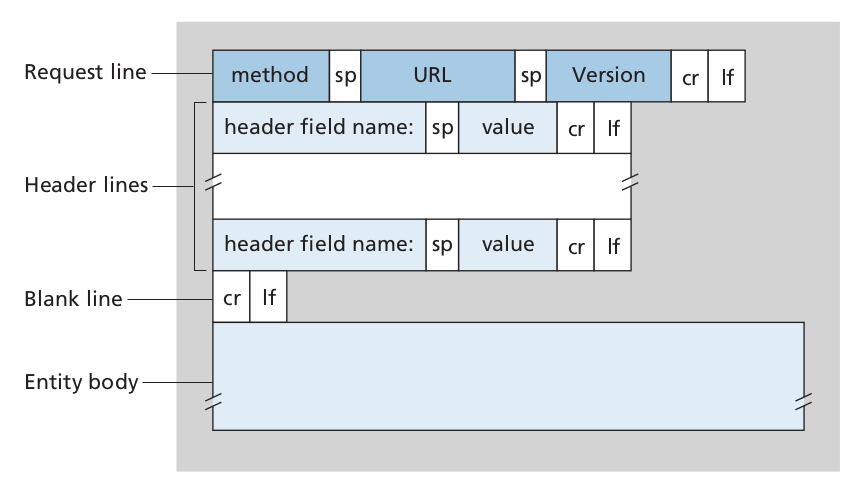
\includegraphics[width=0.5\textwidth]{images/http_request_message.png}
	\caption{Formato generale dei messaggi di richiesta HTTP}
	\label{fig:esempio}
\end{figure}

Il corpo è (solitamente, per convenzione) vuoto nelle richieste GET.

\subsubsection*{Messaggio di risposta HTTP}
Un esempio di messaggio di risposta HTTP è
\\\\
\texttt{HTTP/1.1 200 OK}\\
\texttt{Connection: close}\\
\texttt{Date: 18 Aug 2025}\\
\texttt{Server: Apache}
\texttt{Last-Modified: 11 Jun 2025}
\texttt{Content-Length: 3145}\\
\texttt{Content-Type: text/html}\\
\texttt{<html>...</head>}\\

Troviamo la riga di intestazione, un numero variabile di intestazioni e il corpo.

\begin{itemize}
	\item La riga di stato presenta tre campi: la versione del protocollo, un codice di stato e un messaggio relativo al codice di stato
	\item Connection: close sta ad indicare che il server ha intenzione di chiudere la connessione TCP dopo l'invio del messaggio
	\item Date indica la data di invio del messaggio
	\item Server indica il tipo di server che sta fornendo il messaggio
	\item Last-Modified indica quando l'oggetto è stato modificato per l'ultima volta
	\item Content-Length indica quanti byte è il corpo
	\item Content-Type indica il tipo del corpo, in questo caso un file HTML.
\end{itemize}

\subsection*{2.2.4 Interazione utente-server: i cookie}
Abbiamo detto che HTTP è stateless. Tuttavia, è spesso auspicabile che i web server possano tener traccia degli utenti per limitare l'accesso ad alcune pagine a taluni o per fornire contenuti in funzione della loro identità.

A questo scopo HTTP adotta i cookie, che consentono ai server di tener traccia degli utenti.

Per poter utilizzare i cookie sono necessari 4 componenti:
\begin{itemize}
	\item Una riga di intestazione nel messaggio di risposta
	\item Una riga di intestazione nel messaggio di richiesta
	\item Un file mantenuto sul sistema dell'utente gestito dal browser
	\item Un database sul server
\end{itemize}

Il server crea un identificativo univoco e lo inserisce all'interno del proprio database. A questo punto il server risponde al browser inserendo nel messaggio HTTP un header chiamato Set-cookie che contiene il numero identificativo. Quando il browser riceve il messaggio, aggiunge una riga nel proprio file. Questa riga contiene il nome del server e il numero identificativo.

Ogni volta che l'utente richiede una pagina web, il suo browser consulta il suo file dei cookie, estrae il suo numero identificativo per il sito e lo pone nella richiesta HTTP. In tal modo il server può monitorare l'attività dell'utente nel sito.

\subsection*{2.2.5 Web caching}
Una web cache è un'entità di rete che soddisfa richieste HTTP al posto del web server effettivo. Il proxy ha una propria memoria in cui conserva copie di oggetti recentemente richiesti.

Ecco cosa succede:
\begin{enumerate}
	\item Il browser stabilisce una connessione TCP con il proxy serber e gli invia una richiesta HTTP per l'oggetto specificato.
	\item Il proxy controlla la presenza di una copia dell'oggetto memorizzato localmente. Se l'oggetto viene rilevato, il proxy lo inoltra al client
	\item Se la cache non dispone dell'oggetto, apre una connessione con il server di origine, richiedendo l'oggetto in questione. Il server gli risponde
	\item Il proxy salva l'oggetto nella propria cache e lo manda al client.
\end{enumerate}

Il proxy è contemporaneamente sia client che server a seconda dei casi.

I proxy possono (1) ridurre i tempi di risposta ai client e (2) riducono il carico dei web server e dei loro collegamenti. Ciò implica che l'intero Internet ne trae beneficio.

\subsection*{GET condizionale}
L'oggetto ospitato nel web server potrebbe essere stato modificato rispetto alla copia presente nel proxy. HTTP presenta un meccanismo che permette alla cache di verificare se i suoi oggetti sono aggiornati. Questo meccanismo è chiamato GET condizionle.

Un messaggio di richiesta HTTP viene chiamato messaggio di GET condizionale se (1) usa il metodo GET e (2) include una riga di intestazione If-modified-since.

Vediamone il funzionamento:
\begin{enumerate}
	\item Un proxy invia un messaggio di richiesta a un web server per conto di un browser richiedente, il quale gli risponde.
	\item In cache memorizza sia l'oggetto che la data di ultima modifica presente nell'intestazione Last-Modified
	\item Se dopo un certo periodo di tempo un client richiede la stessa risorsa, la cache non può rispondere direttamente con quella che ha in memoria perché potrebbe essere stata modificata sul server originale. Allora la cache effettua un controllo di aggiornamento inviando una GET condizionale al server, specificando nell'header If-modified-since la data che ha in memoria precedentemente prelevata dall'header Last-Modified. Questo comunica al server di inviare l'oggetto solo se è stato modificato rispetto alla data specificata
	\item Se è stato modificato, il server risponde con un messaggio HTTP normale compreso di oggetto e la cache aggiorna il valore di ultima modifica. Altrimenti manda un messaggio HTTP con corpo vuoto (per non sovraccaricare inutilmente la banda) con messaggio di stato 304 Not Modified che comunica al proxy che può procedere a inoltrare al client la copia dell'oggetto presente in cache
\end{enumerate}

\section*{2.3 Posta elettronica in Internet}
L'email rappresenta un mezzo di comunicazione asincrono.

L'email è composta da tre elementi principali: gli user agent (i programmi di posta), i server di posta e i protocolli quali SMTP, POP e IMAP.

Quando il mittente ha finito di comporre un messaggio, il suo user agent  lo invia al suo server di posta. Se il destinatario ha un altro server di posta, il primo manda il messaggio al secondo. Infine, l'user agent del destinatario recupera il messaggio dal suo server di posta. Ogni utente ha una casella di posta (uno spazio a lui dedicato) su un server di posta su cui vengono depositate le mail a lui indirizzate.

Se il server del mittente non può consegnare la posta a quello del destinatario, la trattiene in una coda dei messaggi e riprova l'invio diverse volte. Dopo averci provato più volte e ogni volta l'invio fallisce, il server del mittente comunica al mittente la mancata consegna.

SMTP presenta il principale protocollo a livello di applicazione per la posta elettronica. Fa uso del protocollo TCP sulla porta assegnata numero 25. Esso presenta un lato client e un lato server. Un server di posta può agire sia da client che da server SMTP: quando la invia agisce come client, quando la riceve agisce come server.

\subsection*{2.3.1 SMTP}
SMTP trasferisce i messaggi dall'user agent del mittente al proprio server, nonché dal server del mitente a quello del destinatario.

Vediamo cosa accade nel dettaglio:
\begin{enumerate}
	\item Il mittente invoca il proprio user agent per la posta elettronica, fornisce l'indirizzo di posta del destinatario, compone il messaggio e dà istruzione allo user agent di inviare il messaggio.
	
	\item Lo user agent invia il messaggio al proprio server di posta tramite SMTP (vedremo più avanti che potrebbe usare anche HTTP)
	
	\item Il lato client di SMTP, eseguito sul server mittente, apre una connessione TCP verso il server SMTP in esecuzione sul mail server del destinatario (se questi usa un server diverso da quello del mittente)
	
	\item Il client SMTP (sul server mittente) invia il messaggio al server SMTP (server ricevente)
	
	\item Il server SMTP del ricevente pone il messaggio nella casella del destinatario
	
	\item Il destinatario, quando lo ritiene opportuno, invoca il proprio user agent per leggere il messaggio (usando POP, IMAP o HTTP che vedremo più avanti)
\end{enumerate}

\begin{figure}[h]
	\centering
	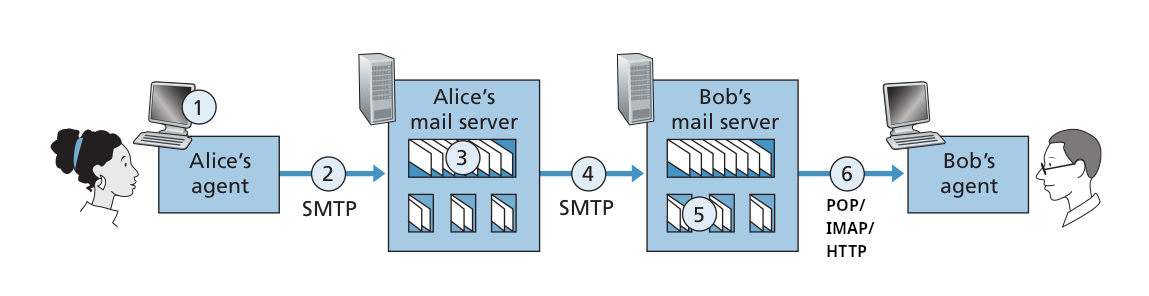
\includegraphics[width=0.5\textwidth]{images/SMTP_example.png}
	\caption{Esempio di funzionamento}
	\label{fig:esempio}
\end{figure}

Il client (o i client) riusano la stessa connessione TCP se hanno altri messaggi da inviare al server, pertanto, SMTP fa uso di connessioni persistenti.

\subsection*{2.3.2 Confronto con HTTP}
HTTP trasferisce i file da un web server a un web client, mentre SMTP trasferisce messaggi di posta elettronica da un mail server a un altro.

Sia HTTP standard che SMTP fanno uso di connessioni persistenti.

Una differenza sostanziale è che HTTP è un protocollo di tipo pull, ovvero il client "tira" le informazioni del server a sè. In altre parole chi instaura la connessione è la macchina che vuole ricevere il file. Al contrario SMTP è un protocollo di tipo push, ovvero il client "spinge" le informazioni al server. In altre parole, la connessione TCP viene inizializzata dall'host che vuole spedire i file.

Un'altra differenza è che SMTP obbliga l'intero messaggio a essere codificato in ASCII a 7 bit mentre HTTP non pone tale restrizione.

\subsection*{2.3.3 Formati dei messaggi di posta}
Il corpo dei messaggi di posta è preceduto da degli header.
Queste righe contengono testo leggibile, costituito da una parola chiave, seguita da due punti a loro volta seguiti da un valore (esempio: Subject: this is an email). Alcune di queste righe sono obbligatorie, come From e To. Attenzione a non confondersi tra i "From/To" dei messaggi SMTP e i "From/To" degli header di messaggio.

\subsection*{2.3.4 Protocolli di accesso alla posta}
Quando SMTP consegna il messaggio alla casella del destinatario, come fa quest'ultimo a recuperare il messaggio? 

Verrebbe quasi naturale rispondere "posizioniamo un server SMTP presso il computer del destinatario", ma con questo approccio il computer del destinatario dovrebbe rimanere sempre acceso e connesso a Internet al fine di ricevere la posta. Ciò non è raccomandabile, pertanto si preferisce che l'utente acceda alla propria posta che risiede sul server quando e come egli vuole. Si noti che non possiamo usare SMTP qui in quanto esso è un protocollo push mentre in questo caso servirebbe un protocollo pull.

Ebbene, si usano dei protocolli per richiedere e trasferire la posta dal server al client. I principali sono POP3, IMAP e HTTP.

Ricapitolando, SMTP è usato per trasferire posta dallo user agent del mittente al proprio server di posta ed è usato per trasferire la posta dal server mittente al server destinatario, ma per trasferire la posta dal server destinatario al suo user agent è necessario un protocollo di accesso alla posta.

\subsubsection*{POP3}
POP3 entra in azione quando lo user agent (il client), apre una connessione TCP verso il mail server sulla porta 110. POP3 procede in tre fasi: autorizzazione, transazione e aggiornamento.

Durante la prima fase lo user agent invia nome utente e password.

Durante la seconda fase lo user agent recupera i messaggi e può marcarne alcuni (anche quelli non scaricati) come da eliminare.

La fase di aggiornamento ha luogo quando il client conclude la sessione e in questo istante il server elimina i messaggi che sono stati marcati come da eliminare.

Uno user agent che usa POP3 può essere configurato dall'utente per "scaricare e cancellare" o per "scaricare e mantenere". Nella modalità scarica e cancella, come suggerisce il nome, il client dice al server di cancellare tutte le mail che ha scaricato. Se ciò avviene, il destinatario non può visualizzare i messaggi da un altro dispositivo.

\subsubsection*{IMAP}
Con l'accesso tramite POP3, dopo aver scaricato i messaggi sulla macchina locale, l'utente può creare cartelle nelle quali inserire i messaggi. Questo paradigma pone però problemi per gli utenti mobili in quanto la struttura delle directory non si muove insieme a loro. Serve allora un modo per mantenere la gerarchia delle cartelle sul server alla quale si può accedere da diversi calcolatori.

Per risolvere questo e altri problemi viene in soccorso il protocollo IMAP. Un server che adotta il protocollo IMAP associa ogni messaggio arrivato al server in una cartella. L'utente può crearne di altre e spostare i messaggi al loro interno. IMAP fornisce anche comani per consentire agli utenti di effettuare ricerche in cartelle remote. Un'altra caratteristica è che consente di scaricare solo singole parti dei messaggi.

\subsubsection*{Posta basata sul Web}
Al giorno d'oggi gli utenti possono inviano e leggono posta su un browser Web. In questo caso lo user agent è un browser web e l'utente comunica con il proprio server web via HTTP.

In ogni caso, anche se gli utenti finali comunicano con i loro server via HTTP, i server tra di loro comunicano via SMTP.

\section*{2.4 DNS: il servizio di directory di Internet}
Gli host di internet possono essere identificati possono essere indentificati in due modi: tramite il nome host (es. www.eff.org), che sono facili da ricordare per le persone ma non adatti per un sistema di routing e tramite indirizzo IP, difficili da ricordare ma adatto per il sistema di routing in quanto otteniamo informazioni più dettagliate all'interno del collocamento della macchina ad esso associato.

Ogni indirizzo IP è formato da 4 byte con un punto che divide ogni byte espresso in decimale da 0 a 255 (es. 192.168.10.255). Gli indirizzi IP sono gerarchici perché leggendoli da sinistra verso destra otteniamo informazioni sempre più specifiche sulla collocazione dell'host all'interno di Internet.

\subsection*{2.4.1 Servizi forniti da DNS}
Come poc'anzi anticipato, le persone prediligono usare un nome host mentre i router prediligono usare un indirizzo IP.

Al fine di conciliare i due approcci, ovvero far usare alle persone l'hostname e ai router l'indirizzo IP, è necessario un servizio che sia in grado di tradurre i nomi degli host nei loro indirizzi IP. Si tratta del compito del DNS. DNS è (1) un database distribuito e (2) un protocollo a livello di applicazione che consente agli host di interrogare il database.

Il DNS usa UDP sulla porta 53 e viene comunemente utilizzato da altri protocolli a livello di applicazione come HTTP e SMTP.

Questo è il funzionamento quando si richiede una pagina Web:
\begin{enumerate}
	\item Il browser estrae il nome dell'host dall'URL e lo passa al lato client dell'applicazione DNS
	\item Il client DNS invia un'interrogazione contenente l'hostname a un server DNS
	\item Il client riceve una risposta che include l'indirizzo IP corrispondente all'hostname
	\item Una volta ricevuto l'indirizzo IP dal DNS, il browser dò inizio a una connessione TCP sulla porta 80 a quell'indirizzo
\end{enumerate}

Pertanto, il sistema DNS aggiunge un ritardo aggiuntivo alle applicazioni Internet che lo utilizzano.

Oltre alla traduzione degli hostname in indirizzi IP, il DNS mette a disposizione altri servizi:
\begin{itemize}
	\item Host aliasing: Un host dal nome complicato (hostname canonico) può avere uno o più sinonimi (alias). Il DNS può essere invocato per ottenere l'hostname canonico da un alias
	\item Mail server aliasing: UGUALE AL PRIMO???
	\item Distribuzione del carico di rete: I siti con molto traffico vengono replicati su più server, ognuno eseguito su un host diverso con un indirizzo IP diverso. Viene dunque associato un hostname a un INSIEME di indirizzi IP. Quando un client effettua una query per questo hostname, il server risponde con l'intero insieme di indirizzi, ma di volta in volta stravolgendone l'ordine. Dato che generalmente un client invia il suo messaggio al primo indirizzo IP elencato, ciò contribuisce a distribuire il traffico su server replicati.
\end{itemize}

\subsection*{2.4.2 Panoramica del funzionamento di DNS}
Tutte le query DNS e i messaggi di risposta vengono inviati all'interno di datagrammi UDP alla porta 53. Il client DNS sull'host riceve un messaggio di risposta contenente la corrispondenza desiderata che viene inoltrata all'applicazione che ne ha fatto richiesta. Pertanto, dal punto di vista dell'applicazione, la risoluzione dell'hostname è una scatola nera.

Per implementare il servizio DNS un primo approccio potrebbe essere quello di creare un DNS server contenente tutte le corrispondenze. Ciò sarebbe inappropriato per i seguenti motivi: un solo punto di fallimento, volume di traffico spropositato per un solo nodo, database geograficamente distante e manutenzione (dovrebbe essere aggiornato frequentemente per tener conto di ogni nuovo host).

\subsubsection*{Un database distribuito e gerarchico}
In realtà il servizio DNS utilizza un gran numero di server, organizzati in maniera gerarchica e distribuiti. Nessun DNS server ha tutte le corrispondenze per tutti gli host di Internet. Questa gerarchia consiste di tre classi di DNS server: i root server, i top-level domain server e i server autoritativi.

Immaginiamo un client che voglia raggiungere www.eff.org. Esso dapprima contatta uno dei root server che gli restituisce uno o più indirizzi IP di server DNS relativi al TLD .org, che a sua volta gli restituisce uno o più server DNS autoritativi per eff.org. A questo punto quest'ultimo restituisce l'indirizzo IP dell'hostname www.eff.org.

Esaminiamo più in dettaglio le varie classi di server DNS:
\begin{itemize}
	\item Root server: ne sono circa 400 in tutto il mondo e forniscono gli indirizzi IP dei TLD DNS Server
	\item TLD server: Questi server si occupano dei domini di primo livello quali org, com, edu, it, fr ecc. Questi forniscono gli indirizzi IP dei server autoritativi
	\item Server autoritativi: Ogni organizzazione dotata di host pubblicamente accessibili su Internet deve fornire record DNS pubblicamente accessibili che associno i nomi di tali host a indirizzi IP.
\end{itemize}

Esiste un altro tipo di server DNS detto DNS server locale, che non appartiene alla gerarchia di server sopra descritta. Ciascun ISP ha un proprio DNS server locale, fornito ai clienti che vi si connettono. Quando un host effettua una richiesta DNS, la query viene inviata al DNS server locale, che opera da proxy e inoltra la query alla gerarchia DNS.

Il funzionamento per risolvere www.domain.it è il seguente:
\begin{enumerate}
	\item L'utente invia una richiesta DNS al server locale
	\item Il server locale inoltra la query al root server, che, vedendo che il TLD è .it, risponde con uno o più indirizzi IP appartenenti ai TLD server inerenti .it
	\item Il server locale, dunque, invia la richiesta a uno dei TLD server che risponde con uno o più indirizzi IP di DNS server autoritativo per domain.it
	\item Il DNS server locale, annotato ciò, invia la richiesta a uno di questi, il quale risponde con l'indirizzo IP dell'hostname finale
	\item Il DNS server locale inoltra questa informazione all'host richiedente.
\end{enumerate}

\begin{figure}[h]
	\centering
	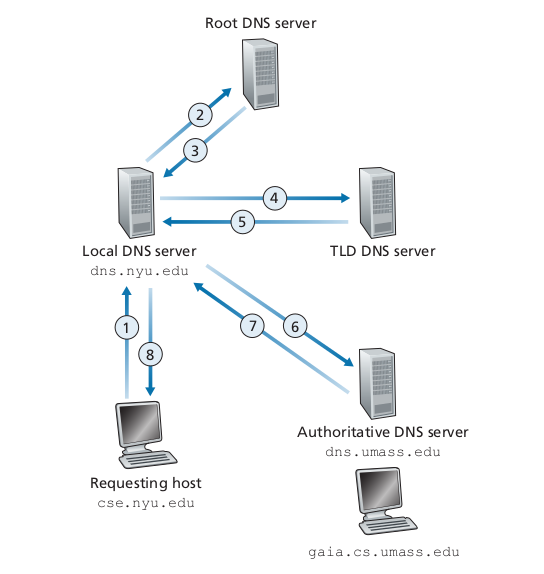
\includegraphics[width=0.5\textwidth]{images/dns_query_example.png}
	\caption{Esempio di funzionamento}
	\label{fig:esempio}
\end{figure}


In questo esempio si fa uso sia di query ricorsive che di query iterative. La richiesta effettuata dal client al DNS server locale è ricorsiva in quanto il client chiede a quest'ultimo di ottenere l'associazione dell'hostname (cioè non rimbalza al client un risultato intermedio che ha trovato). Tutte le altre richieste sono iterative in quanto server A chiede a B di risolvere solo una parte dell'hostname. Server B gli risponde e sarà compito di A procedere nella ricerca. Ogni richiesta DNS può essere o iterativa o ricorsiva.

\subsubsection*{DNS caching}
In una concatenazione di richieste il server DNS che riceve una risposta da un altro server DNS può mettere in cache le informazioni ricevute, in modo che possa rispondere senza interrogare altri server e conseguentemente incrementare i ritardi. Dopo un determinato periodo di tempo i server DNS svuotano l'informazione ricevuta. Ad esempio un DNS server locale può memorizzare in cache l'indirizzo IP dei TLD DNS server, aggirando la richiesta ai root DNS server.

\subsection*{2.4.3 Record e messaggi DNS}
Il database DNS contiene i cosiddetti resource record, che sono restituiti alle richieste DNS.


Un record di risorsa contiene i seguenti campi: (Name, Value, Type, TTL).

Il TTL è il time to live e indica quanto tempo residuo in cache prima di essere rimosso. Il significato di Name e Value dipende da Type.
\begin{itemize}
	\item Se Type=A allora Name è il nome dell'host e Value è il suo indirizzo IP. Pertando un record di tipo A fornisce la corrispondenza tra hostname e indirizzo IP
	\item Se Type=NS allora Name è un dominio e Value è l'hostname del DNS server autoritativo [ma non era un IP???]
	\item Se Type=CNAME allora Name è l'alias e Value è il nome canonico
	\item Se Type=MX allota Value è il nome canonico di un mail server che ha Name come alias (???? allora è uguale a CNAME ????)
\end{itemize}

Ogni server DNS autoritativo contiene un record A per un certo hostname ma anche un altro tipo di server DNS può contenere record A nella propria cache.

\subsubsection*{Messaggi DNS}
Sia le query che le risposte hanno lo stesso formato
\textbf{DA COMPLETARE}

\subsubsection*{Inserimento di un record nel database DNS}
Come vengono inseriti i record nel database DNS? Un utente che vuole registrare un nome di dominio deve rivolgersi presso un registrar che si occupa di verificare l'unicità del nome di dominio e di inserirlo nel database DNS. Quando l'utente registra un nome di dominio presso un registrar bisogna fornirgli anche i nomi e gli indirizzi IP dei DNS server autoritativi.

Fino a poco tempo fa i contenuti di ciascun server DNS venivano inseriti in maniera statica per mezzo di un file di confiurazione. Con le nuove versioni del protocollo DNS è stata aggiunta l'opzione UPDATE per consentire l'aggiunta o la cancellazione dinamica dei dati del database attraverso messaggi DNS.




























































































\end{document}